\begin{section}{biased-ciphertext attack}
\label{sec:biased_ciphertext}

\begin{figure}[!ht]
	\centering
	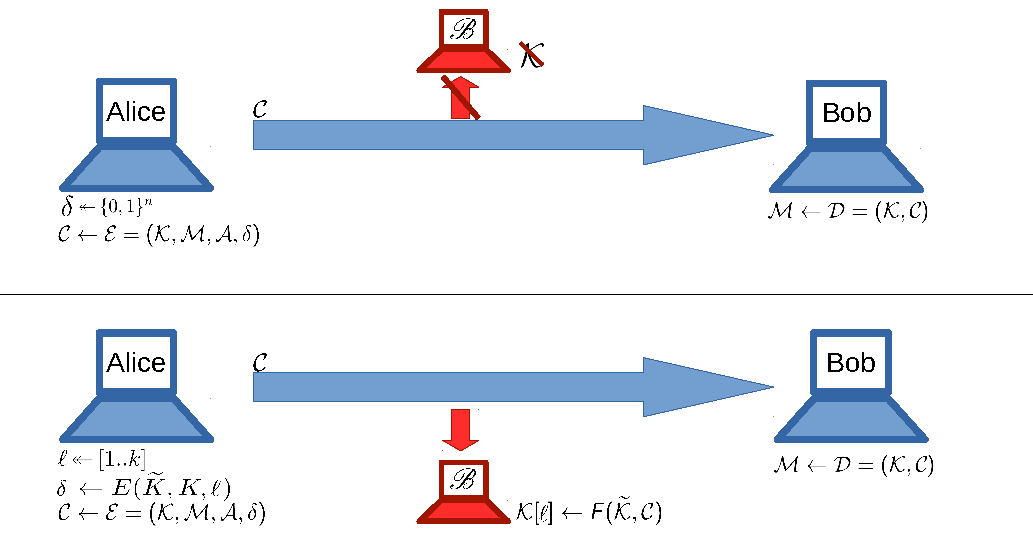
\includegraphics[width=\textwidth]{image/biased_ciphertext}
	\caption{biased-ciphertext attack.}
	\label{fig:biased_ciphertext}
\end{figure}


\begin{subsection}{Grundidee}

Die vorherigen Angriffe sind nur anwendbar auf spezielle Klassen von symmetrischen Verschlüsselungen. Ein universeller Ansatz für eine $ASA$ ist die biased-ciphertext attack. In diesem Fall kann ein symmetrisches Schema ohne öffentlicher nonce angegriffen werden. Ziel sind symmetrische stateless Schemen mit kleiner Zufallskomponente. Bitweise werden Teile von $\mathcal{K}$ über den Chiffretext $\mathcal{C}$ selbst hinweg verraten.

\end{subsection}

\begin{subsection}{Durchführung}

Entscheidend bei diesem Angriff ist, dass kein öffentlicher nonce nötig ist. Wie auf Abbildung \ref{fig:biased_ciphertext} zu sehen, wurde zum Verschlüsseln auf Alices Seite ein Zufall $\delta$ verwendet. Wie der IV in den vorherigen Angriffen, beinhaltet $\delta$ nicht verifizierbaren Zufall und der eigentliche Zufallszahlengenerator kann gegen die Funktion $E$ ausgetauscht werden. Diese verwendet den Masterschlüssel $\widetilde{\mathcal{K}}$ um ein zufälliges Bit $\ell$ des geheimen Schlüssels $\mathcal{K}$ in dem jetzt nicht mehr ganz zufällig gewählten $\delta$ zu verstecken. Die Funktion $\mathcal{E}$ verwendet $\delta$ anschließend um den Chiffretext zu erzeugen. Big Brother ist nun in der Lage, mit Hilfe von $\widetilde{\mathcal{K}}$ und einer Funktion $F$ bitweise den geheimen Schlüssel $\mathcal{K}$ zu reproduzieren. Wenn so nur ein einziges Bit $\ell$ von $\mathscr{B}$ errechnet werden kann, werden nur $|\mathcal{K}|$ Verschlüsselungen benötigt, um den vollständigen Schlüssel $\mathcal{K}$ zu bestimmen. Die Autoren legen Wert darauf, dass dies keine chosen-message attack ist. Big Brother kann den geheimen Schlüssel zurückrechnen, unabhängig von der Nachricht $M$ oder der assoziierten Daten $A$. Es benötigt lediglich $|K|$ Verschlüsselungen für ein key recovery. Essentiell wichtig hierbei ist, dass das Tupel $(\mathcal{K}, \mathcal{M}, \mathcal{A}, \delta)$ injektiv zum Chiffretext $\mathcal{C}$ ist. Diese Bedingung schränkt die angreifbaren Schemen allerdings nicht sehr ein, denn auch auf Schemen mit öffentlich übertragenen IV trifft diese Bedingung zu.

\end{subsection}

\begin{subsection}{Entdeckbarkeit}

So lange die Subversion genügend Zufall verwendet, zum Beispiel mehr als sieben Bit, ist die Subversion unentdeckbar. Aber auch hier gilt: Ein Reset des Systems erhöht die Wahrscheinlichkeit sie zu entdecken.

\end{subsection}

\end{section}
